% Created 2022-06-03 Fri 10:48
% Intended LaTeX compiler: pdflatex
\documentclass[11pt]{article}
\usepackage[utf8]{inputenc}
\usepackage[T1]{fontenc}
\usepackage{graphicx}
\usepackage{longtable}
\usepackage{wrapfig}
\usepackage{rotating}
\usepackage[normalem]{ulem}
\usepackage{amsmath}
\usepackage{amssymb}
\usepackage{capt-of}
\usepackage{hyperref}
\usepackage{cleveref}
\usepackage{subfig}
\usepackage[letterpaper, margin=1in]{geometry}
\usepackage{fancyhdr}
\pagestyle{fancy}
\usepackage{amssymb}
\usepackage[citestyle=authoryear,bibstyle=authoryear, hyperref=true,backref=true,maxcitenames=3,url=true,backend=biber,natbib=true] {biblatex}
\addbibresource{export/bibs.bib}
\fancyhead[CO,CE]{\textbf{[Align-BDD]}}
\fancyhead[LO,LE]{A.B.}
\fancyhead[RO,RE]{Application: j-UFLP.}
\author{Alexey Bochkarev}
\date{\today}
\title{Align-BDD application: on joint UFLP.}
\hypersetup{
 pdfauthor={Alexey Bochkarev},
 pdftitle={Align-BDD application: on joint UFLP.},
 pdfkeywords={},
 pdfsubject={},
 pdfcreator={Emacs 29.0.50 (Org mode 9.5.2)}, 
 pdflang={English}}
\begin{document}

\maketitle
\section{Summary and questions TBD}
\label{sec:org27bdc3e}
\begin{itemize}
\item weak point: CPP MIP
\item weak point: feeding more info to the DD-based methods.
\item weak point: not that much variety in graph topologies.
\item question: not equivalent to another UFLP? I guess not (consider j10 and j16).
\end{itemize}

\section{Joint-UFLP formulation}
\label{sec:jUFLP}
We next illustrate the performance of our algorithms in the context of a
specific application. We will consider the following variant of the
uncapacitated facility location problem, UFLP \citep{owen1998,revelle2008}, which
we call the ``joint uncapacitated facility location problem,'' j-UFLP. We have
designed this problem specifically to highlight a possible application of our
heuristic. Therefore, it comprises two interconnected, but comparable
subproblems, which can be represented as BDDs.

To introduce j-UFLP, let us first consider a simple UFLP formulation. This
problem considers a set of \(N\) points. At each point \(i\), we can locate a
facility at a cost given by \(c_i\), covering all points in a set given by \(S_i\),
where \(i \in S_i\). (Set \(S_i\) might refer to customers that are sufficiently
close to location \(i\) according to some specified metric, like distance or
travel time.) We also define a cost function \(f_i:
\mathbb{N}_0\rightarrow\mathbb{R}\), so that \(f_i(a)\) would indicate a cost of
covering point \(i\) exactly \(a_i\) times. Note that we do not imply any properties
of \(f_i\), such as convexity or concavity. This UFLP variant minimizes the total
cost and can be formulated as follows:

\begin{subequations}\label{eq:UFLP}
\begin{align}
  \min & \sum_{i=1}^N \Big(c_i x_i + f_i(a_i)\Big)&\\
    \textrm{s.t. } & a_i = \sum_{j\in S_i} x_i& \textrm{ for all } i=1,\ldots, N,\\
    & x_i\in\{0,1\} & \textrm{ for all } i=1,\ldots,N.
\end{align}
\end{subequations}

In our numerical experiments, we consider j-UFLP, which comprises two such
problems, interconnected by having certain common variables. For a set of common
variables  \(J\subseteq\{1,\ldots,N\}\), the j-UFLP is formulated as follows:

\begin{subequations}\label{eq:j-UFLP}
\begin{align}\tag{j-UFLP}
  \min & \sum_{i=1, t=1,2}^N \Big(c^t_i x^t_i + f^t_i(a^t_i)\Big)&\\
    \textrm{s.t. } & a^t_i = \sum_{j\in S^t_i} x^t_i& \textrm{ for all } i=1,\ldots, N, t=1,2,\\
    & x^t_i\in\{0,1\} & \textrm{ for all } i=1,\ldots,N, t=1,2,\\
    & x^1_j = x^2_j & \textrm{ for all } j\in J.\label{eq:link}
\end{align}
\end{subequations}

Further, to make this problem hard for an MIP solver, we induce the following
special structure for the underlying graph. We assume that each sub-problem
graph consists of \(n\) subgraphs, \(M\) nodes each, and that there is at most one
arc between every two subgraphs. Moreover, we assume \(J\) to be the set of
endpoints of such arcs between the subgraphs. An example of such instance is
presented in Figure \ref{fig:sample-jUFLP}. A subgraph corresponding to the first
subproblem is depicted with thick black lines, while the one corresponding to
the second subproblem has thin red lines. Nodes that are common for the two
subgraphs (corresponding to conditions \eqref{eq:link}) are marked with background
color (nodes \texttt{j1}, \texttt{j6}, \texttt{j10}--\texttt{j12}, \texttt{j16}, \texttt{j19}, and \texttt{j21}). Note that
overlaps are calculated independently: e.g., locating a facility at \texttt{j10} does
contribute to \(a_{16}^2\), but not \(a_{16}^1\).

  \begin{figure}%
    \centering
    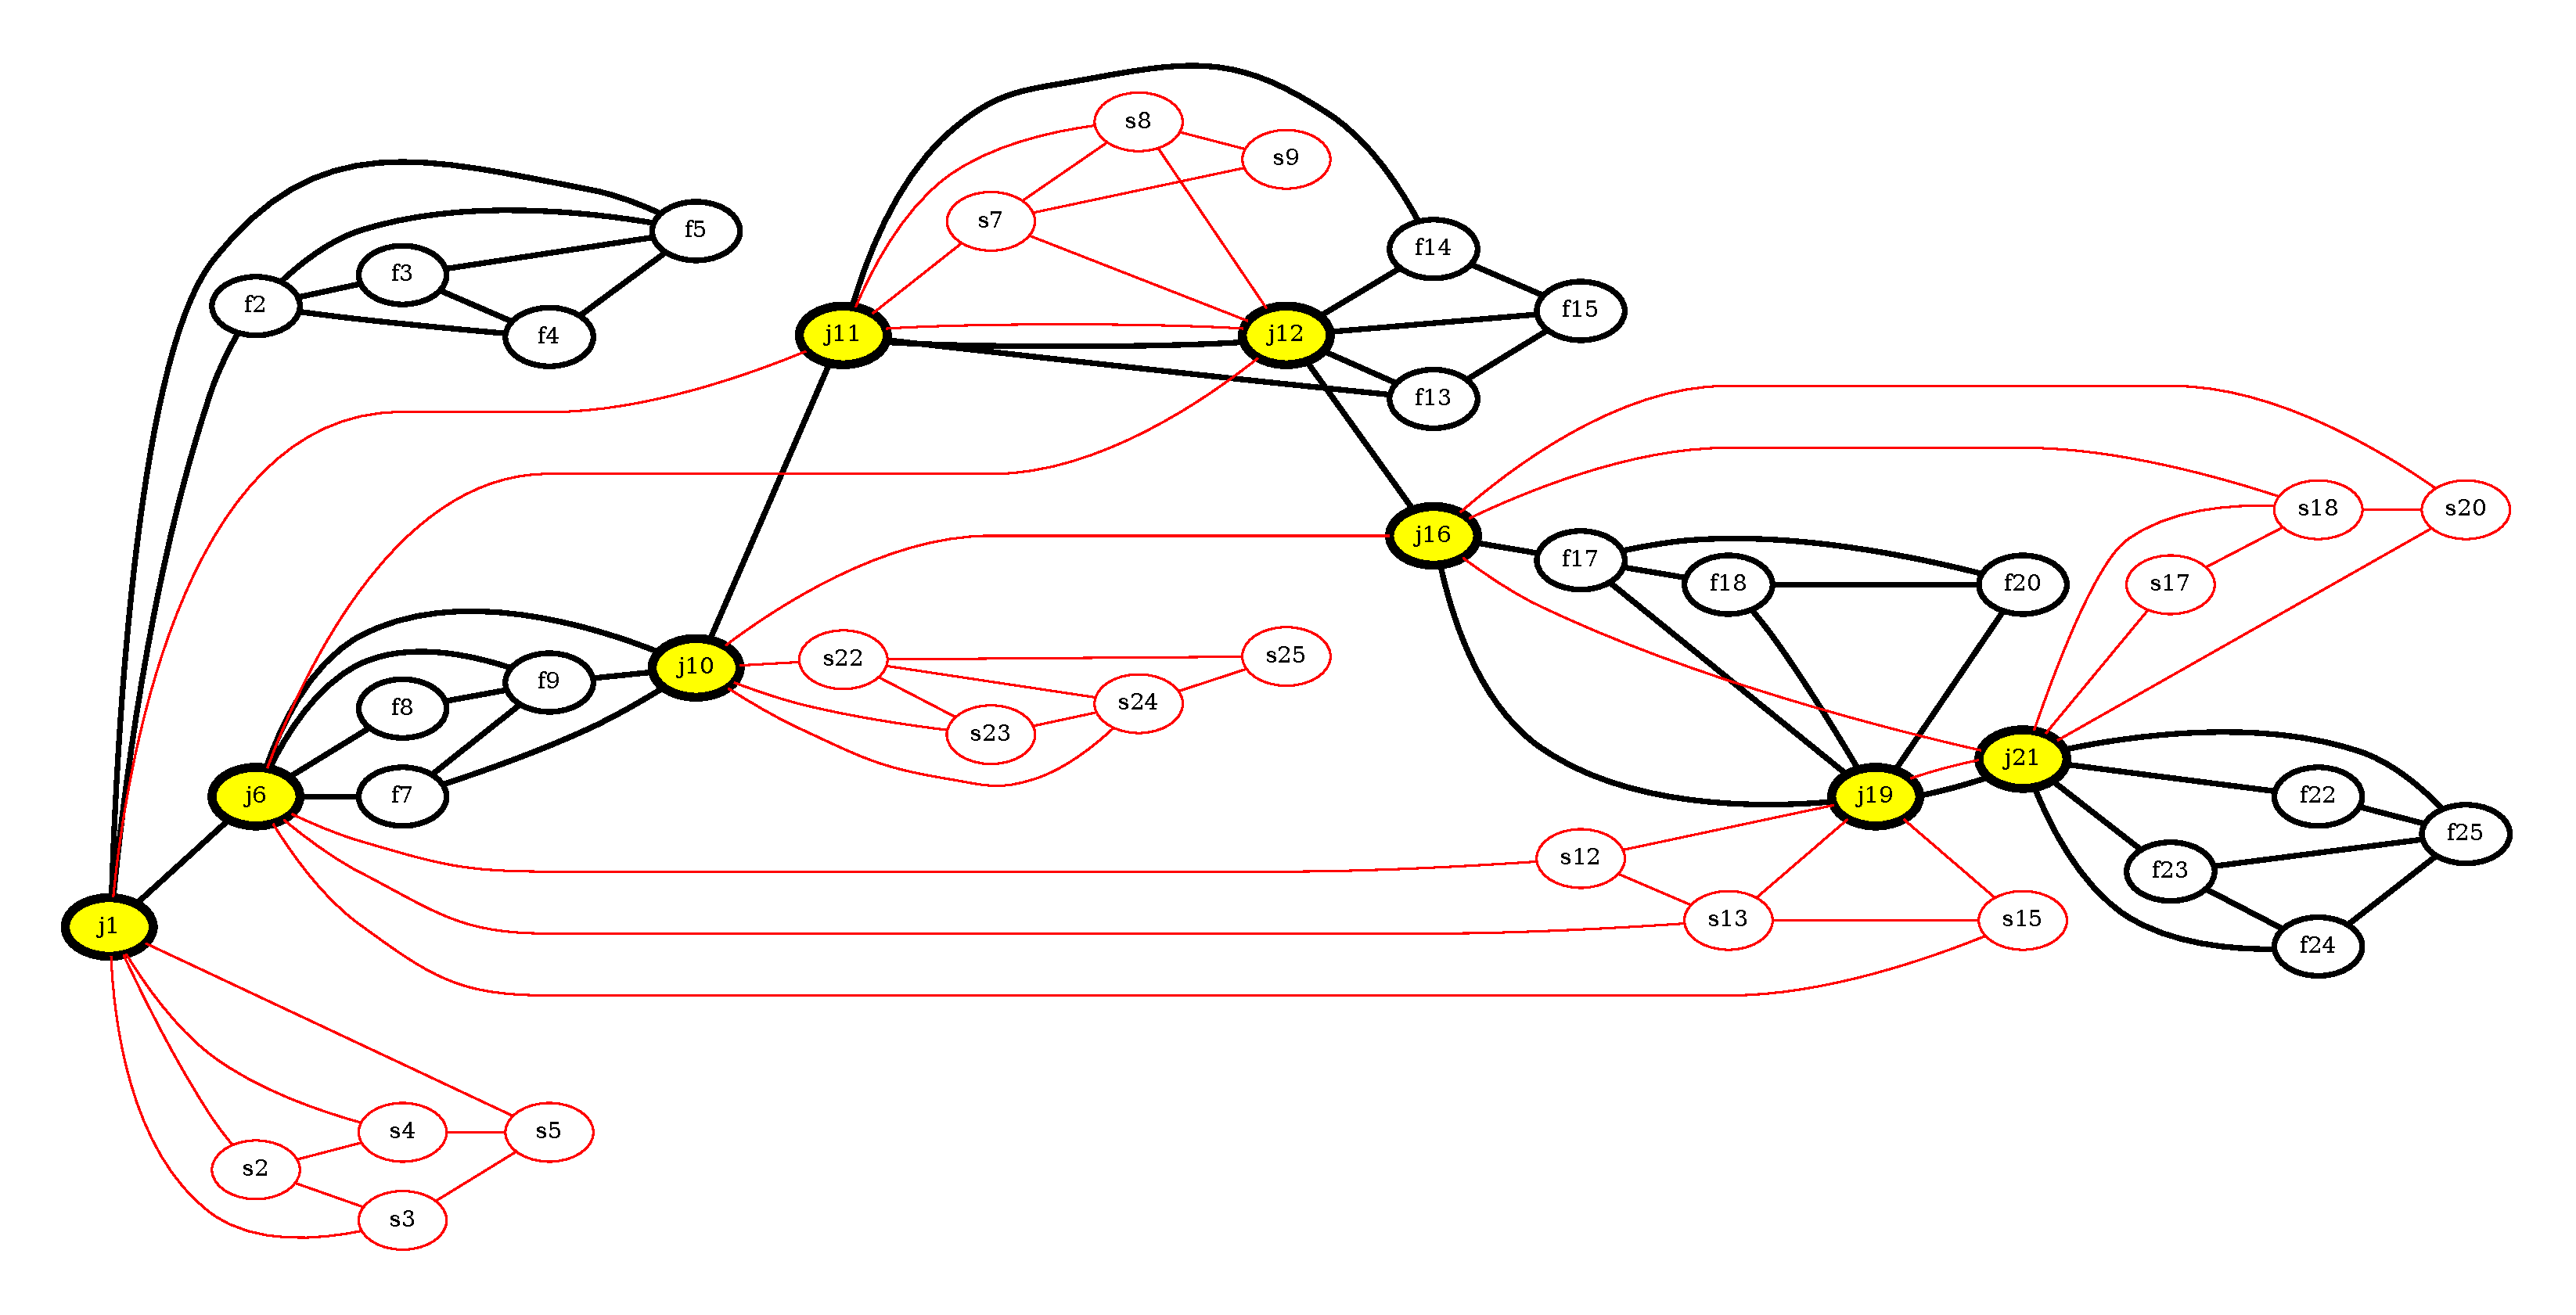
\includegraphics[width=\textwidth]{./sample_jUFLP.pdf}%
    \caption{Sample j-UFLP instance graph.}%
    \label{fig:sample-jUFLP}%
\end{figure}

A naive MIP reformulation for \eqref{eq:j-UFLP} implies introducing new binary
variables \(y_{i,a}^t\) indicating whether point \(i\) in subproblem \(t\) was covered
at least \(a\) times. Therefore, the equivalent problem is:

\begin{subequations}\label{eq:j-UFLP-MIP}
\begin{align}\tag{j-UFLP-MIP}
  \min & \sum_{i=1, t=1,2}^N \Big(c^t_i x^t_i + \sum_{a=0}^{|S_i^t}q_{i,a}^t y^t_{i,a}\Big)+C&\\
    \textrm{s.t. } & \sum_{a=1}^{|S_i|} y_{i,a}^t = \sum_{j\in S^t_i} x^t_i& \textrm{ for all } i=1,\ldots, N, t=1,2,\\
    & y^t_{i,a} \geq y^t_{i, a+1} & \textrm{ for all }i=1, \ldots, N, t=1,2, a=0,\ldots,|S_i|,\\
    & x^t_i\in\{0,1\} & \textrm{ for all } i=1,\ldots,N, t=1,2,\\
    & x^1_j = x^2_j & \textrm{ for all } j\in J,\label{eq:link}
\end{align}
\end{subequations}
where \(q_{i,a}=f_i^t(a)-f_i^t(a-1)\) and \(C=\sum_{i,t} f_i^t(0)\) are constants.

\section{Numerical performance}
\label{sec:orgc3838e4}

  \begin{figure}%
    \centering
    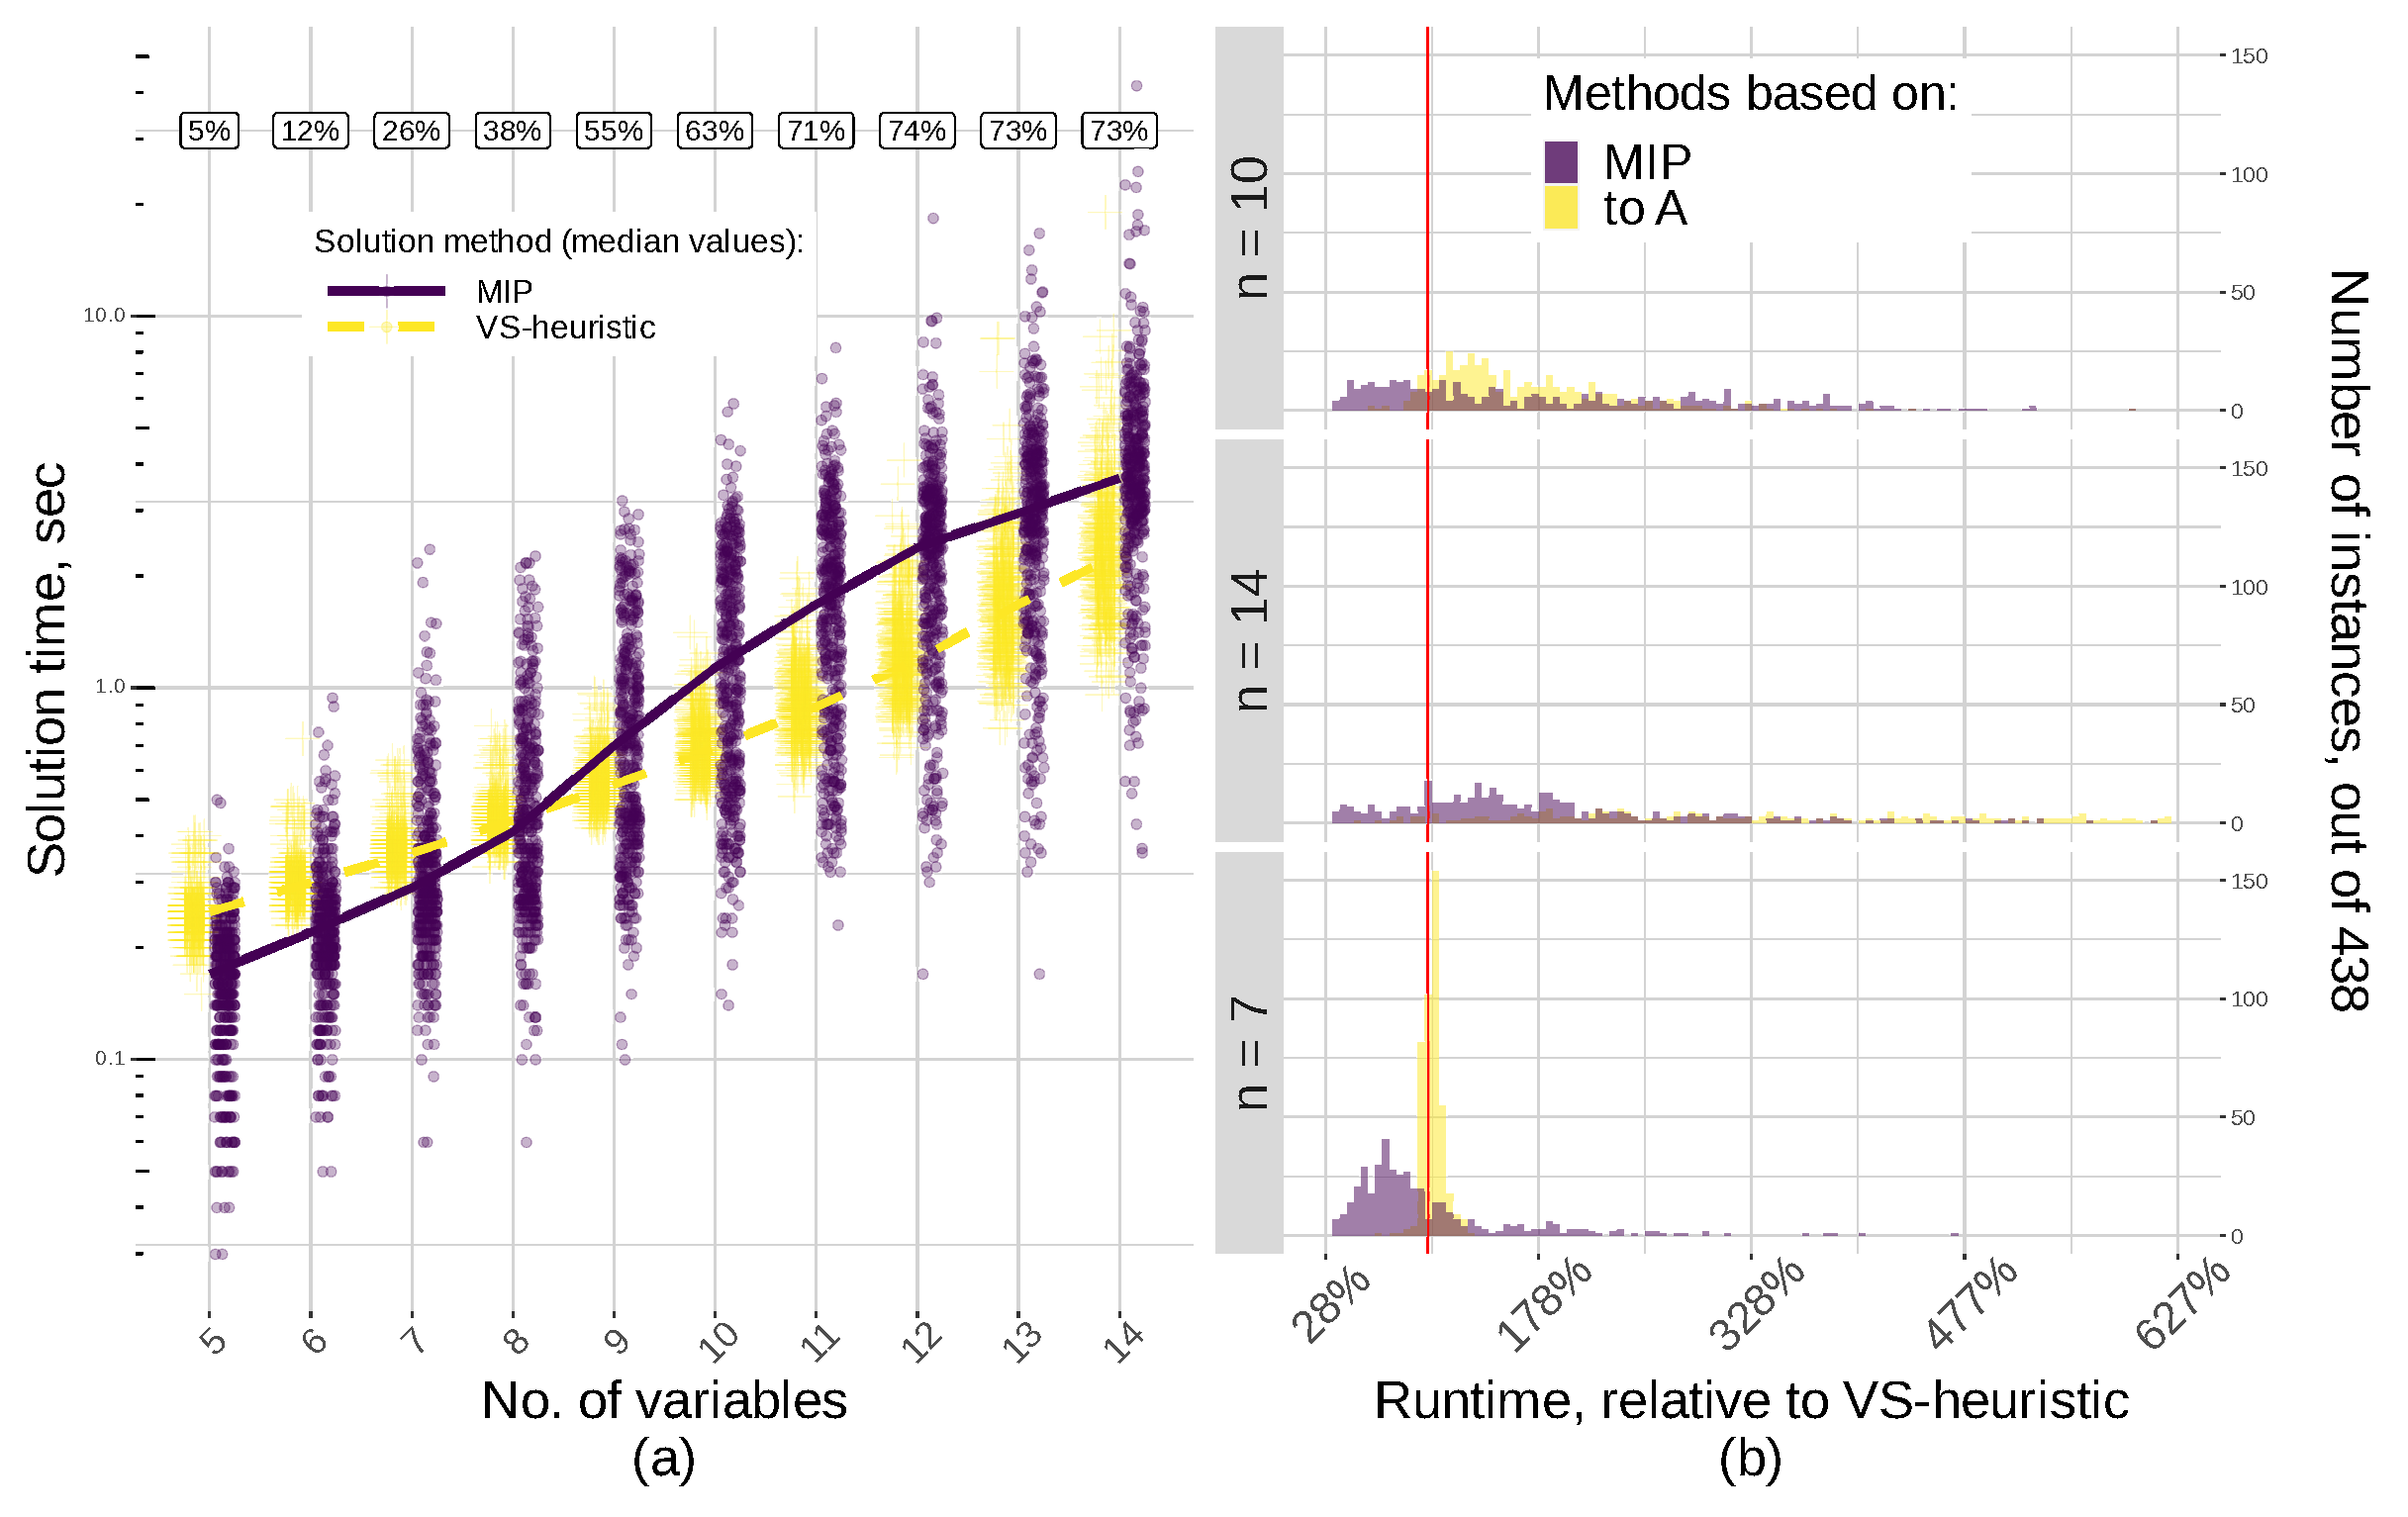
\includegraphics[width=\textwidth]{./jUFLP.eps}%
    \caption{Numerical performance of various heuristics for j-UFLP.}%
    \label{fig:jUFLP-nums}%
\end{figure}
\section{References}
\label{sec:org38a7a76}
\printbibliography
\end{document}